\chapter{Fingerprinting techniques}\label{sec:Fingerprinting}
Fingerprinting is a technique that embeds a piece of information into the data to provide the identification of the owner of data and the source of potential unauthorised data leakage. 
Fingerprint combines secret owner-specific and buyer-specific information and is embedded in the dataset. 
Every buyer has her fingerprint, therefore every dataset fingerprinted and distributed by the owner is different from each other.
By detecting the fingerprint within the dataset, the owner can trace the buyer of that instance of the dataset. 
The fingerprinting techniques usually contain two main algorithms: fingerprint insertion and fingerprint detection. 
In the fingerprint insertion, the fingerprint of a buyer is embedded into the dataset.
Fingerprint detection strives for detecting the fingerprint in a suspicious dataset to connect it with the buyer who distributed the dataset without the authorisation.
Detection could be disrupted by malicious attempts of the buyer to remove the fingerprint from the data, but also by benign changes in the dataset. 
These attacks and fingerprint resistance to them will be addressed in \Cref{sec:Robustness}.


\section{Notation and parameters}
In the following, several different fingerprinting techniques are discussed in detail. 
In this section, we set the common notation and explain the parameters used in the techniques. 
The dataset schema is denoted by $\mathcal{R}(P,A_0,...,A_{v-1})$ where $\mathcal{R}$ is a database relation, \textit{P} is the primary key attribute, and $A_0,...,A_{v-1}$ are $v$ attributes that will be used for fingerprinting. 
$\eta$ is a notion of number of tuples (rows/entries) in the dataset. 
As the fingerprinting techniques embed the fingerprint by changing the attribute values, we define the parameter $\xi$ which denotes the number of least significant bits (LSBs) that can be used to embed the fingerprint. \\
Let \textit{N} be the number of buyers to whom the dataset is being distributed. 
To each of the buyers, a unique fingerprint will be assigned. 
Every fingerprint $\Gamma = (f_0,...,f_{L-1})$ is a binary string of length $L \geq logN$. \\
Besides the buyer's fingerprint, the owner-specific information has to be embedded in the dataset to ensure the ownership protection and make it possible only for the data owner to detect the fingerprint from the fingerprinted dataset. 
This information is usually a secret key $\mathcal{K}$ - a binary string known only to the dataset owner.
\Cref{table:notation} contains the notation that will be used in the remainder of this thesis unless otherwise stated.

\begin{table}
\centering
\caption{The notions of the most common parameters}
\label{table:notation}
\begin{tabular}{|c | c|} 
 \hline
 Notation & Meaning \\ 
 \hline\hline
 $\mathcal{R}$ & database relation \\
 \hline
 \textit{P} & primary key attribute \\
 \hline
 $A_i$ & attribute $i$ \\
 \hline
 \textit{v} & number of attributes \\
 \hline
 $\eta$ & number of tuples  \\
 \hline
 $\mathcal{K}$ & owner's secret key  \\
 \hline
 $\xi$ & number of least significant bits \\ 
 \hline
 $1/\gamma$ & ratio of tuples to be marked\\
 \hline
 \textit{N} & number of buyers \\
 \hline
 \textit{L} & length of fingerprint \\
 \hline
 $\omega_i$ & number of embeddings of a fingerprint bit $i$ \\
 \hline
 $\omega$ & total number of marks \\
 \hline
\end{tabular}
\end{table}

\section{Prerequisites}
Before discussing the specific schemes and algorithms used for fingerprinting relational databases, it is necessary to mention auxiliary functions and algorithms required to achieve the goal of robust fingerprints. 
Cryptographic pseudo-random sequence generator and cryptographic hash function, discussed in the following subsections, both ensure that neither the fingerprint nor any part of fingerprinting scheme get disclosed or recreated by an unauthorised user.
This stated, their usage is crucial for the owner's rights protection.

\subsection{Cryptographic pseudo-random sequence generator}
A cryptographically secure pseudorandom number generator (CSPRNG) is an algorithm for creating a sequence of random numbers with properties suitable for use in cryptography.
The CSPRNG-generated sequence is not truly random, because it is completely determined by the initial value called \textit{seed}. 
The requirements of CSPRNG fall into two groups: 
\begin{itemize}
    \item They pass statistical randomness tests. 
    
    A generator passing the \textit{next-bit test} will pass all other polynomial-time statistical tests for randomness (proof by Andrew Yao in 1982 \cite{yao1982theory}). We say that a sequence of bits passes the next-bit test for at any position $i$ in the sequence, if any attacker who knows the $i$ first bits (but not the seed) cannot predict the $(i+1)$st with reasonable computational power.
    
    \item They resist a serious attack, even when part of their initial or running state becomes available to an attacker.
    
    If part or all of CSPRNG's state has been revealed (or guessed correctly), it should be impossible to reconstruct the stream of random numbers before the revelation. Additionally, if there is an entropy input while running, it should be unfeasible to use knowledge of the input's state to predict future conditions of the CSPRNG state.
\end{itemize}

There is several designed practical CSPRNGs including the Yarrow Algorithm \cite{kelsey1999yarrow} incorporated in iOS and macOS, its successor Fortuna \cite{ferguson2015generating} used in FreeBSD, CryptGenRandom \cite{cryptgenrandom} included in Microsoft's Cryptographic Application Programming Interface, etc.

For the analysis in the thesis, we denote CSPRNG with $\mathcal{S}$, where $\mathcal{S}_i$ denotes the $i^{th}$ random number of the sequence.

\subsection{Cryptographic hash function}
The cryptographic hash function is a deterministic function that takes a string input of any length and returns a fixed-size string value. 
The returned value is called "hash value". 
In literature the hash value can be also referred to as "digest", "checksum" or "digital fingerprint" (the word \textit{fingerprint} is here used in the different context than the \textit{fingerprint} used as a topic of this thesis).
The hash function has three main properties:
\begin{itemize}
    \item It is easy to calculate a hash value for any given input string.
    \item It is computationally difficult to calculate an input that has given a certain hash value.
    \item It is extremely unlikely that two different inputs, even remotely different, have the same hash value.
\end{itemize}

While the regular hash functions aim to, most importantly, avoid the collision of hash values for non-malicious input, the above properties are much strongly guaranteed for cryptographic hash functions.  
The hash value serves as a "signature" for the input provided.
Only the person knowing the original input value can easily check the matching hash function. 
However, knowing only the hash value, one is unable to do the inverse and find out the original input value. 
If either finding a string that matches a given hash value or finding two different inputs that have the same hash value is computationally feasible, then a cryptographic function is not considered secure from a cryptographic point of view.

Most commonly used cryptographic hash functions are MD5 \cite{rivest1992md5} and SHA-1 \cite{eastlake2001us}.


\section{Fingerprint codes}
A fingerprinting scheme assigns a specific fingerprint to each of the \textit{N} buyers.
A fingerprint is a unique binary string of length \textit{L} known only by the database owner which is used to trace a specific owner. 
Storing the mapping of a recipient to her fingerprint is additional data that requires additional protection measures to be protected against attacks.  
To avoid this, the owner uses a cryptographic hash function $\mathcal{H}$ to produce each buyer's fingerprint instead.
In the fingerprinting techniques presented in the following sections, each fingerprint $\mathcal{F}$ is produced as a hash value of the concatenation of owner's secret key $\mathcal{K}$ and buyer's identification number \textit{id}:
\begin{equation}
    \mathcal{F}(\mathcal{K},id)=(f_0,...,f_{L-1})=\mathcal{H}(\mathcal{K}|id)
\end{equation}
where buyer's identification number can be publicly accessible.
This way only the owner who knows both secret key $\mathcal{K}$ and identification number \textit{id} can produce the hash value - the fingerprint of a specific buyer.

\paragraph{Collusion resistant codes}
Fingerprinting schemes are susceptible to collusion attacks where users with multiple copies of the same dataset but different embedded fingerprints work in coalition to create a useful data copy that does not implicate any member of the coalition. 
Collusion attacks will be thoroughly discussed in \Cref{subsec:collusion}, while in this section we cover collusion resistant codes.
Collusion resistant fingerprinting codes have been studied extensively in the literature \cite{boneh1998collusion, guth1999error, pfitzmann1999coin, pfitzmann1996asymmetric, yacobi2001improved}. 
One of the well-known codes is proposed by Boneh and Shaw \cite{boneh1998collusion} (this code is referred to as \textit{BoSh code} in the remainder of the thesis). 
The effectiveness of the BoSh code relies on the assumption that colluding buyers can detect only the fingerprint bits in which their copies differ, otherwise a fingerprint bit cannot be detected.
For example, two buyers with their own fingerprinted datasets can easily compare their datasets and remove or change the values that differ between their copies. 
Authors of \cite{boneh1998collusion} call refer to this as the "Marking Assumption". 
The main property that codes should satisfy is that users cannot change the state of an undetected bit without rendering the dataset useless. 
This small amount of information where the buyers' marks agree is used to trace the copies they generate back to either of them.
A collusion resistant code is expected to have two properties well-elaborated:
\begin{itemize}
    \item $c$-frameproof code, i.e. a coalition of at most $c$ users cannot frame a user not in the coalition even all user fingerprints are known to the users
    \item $c$-secure code, i.e. there exists a tracing algorithm that on input $x$ must output a single member of the coalition of at most $c$ users, where the input $x$ is the new mark extracted by the fingerprint extraction algorithm that was generated by the coalition
\end{itemize}
The usage of the BoSh code is discussed in \Cref{subsec:ak} as a part of the collusion-resistant version of the scheme. 

\section{AK Scheme}\label{subsec:ak}

\begin{algorithm}
  \KwIn{dataset $\mathcal{R}$ with scheme $(P, A_{0}, ..., A_{v-1})$, buyer $n$'s ID $id$}
  \KwOut{fingerprinted dataset $\mathcal{R'}$}
  fingerprint of buyer $n$: $\mathcal{F}(\mathcal{K},id)=\mathcal{H}(\mathcal{K}|id)$
  \\
  \ForEach{tuple $r \in \mathcal{R}$}
  {
    \If{$(\mathcal{S}_{1}(\mathcal{K}|r.P)$ mod $\gamma == 0)$}{
        attribute\_index $i = \mathcal{S}_2(\mathcal{K}|r.P)$ mod $v$
        \\
        bit\_index $j=\mathcal{S}_3(\mathcal{K}|r.P)$ mod $\xi$
        \\
        mask\_bit $x=0$ if $\mathcal{S}_4(\mathcal{K}|r.P)$ is even; $x=1$ otherwise
        \\
        fingerprint\_index $l=\mathcal{S}_5(\mathcal{K}|r.P)$ mod $L$
        \\
        fingerprint\_bit $f=f_l$
        \\
        mark\_bit $m=x \oplus f$
        \\
        $LSB(j,r.A_i) = m$
    }
  }
  \Return{$\mathcal{R'}$}
  \caption{AK Scheme: Insertion Algorithm}
  \label{alg:AK-insertion} 
\end{algorithm}

\begin{algorithm}
  \KwIn{fingerprinted dataset $\mathcal{R'}$ with scheme $(P, A_0, ..., A_{v-1})$}
  \KwOut{suspected buyer's ID $id$}
  //initiate fingerprint template and counts \\
  fingerprint template $\mathcal{F}=(f_0,...,f_{L-1})=(?,...,?)$ // '?' represents unknown value \\
  \For{$i=0$ to $L-1$}
  {
    $count[i][0]=count[i][1]=0$ \\
    // $count[i][0]=count[i][1]$ are votes for $f_i$ to be 0 and 1 respectively
  }
  //scan all tuples and obtain counts for each fingerprint bit \\
  \ForEach{tuple $r \in R'$}
  {
    \If{$\mathcal{S}_1(\mathcal{K},r.P)$ mod $\gamma==0$}
    {
        attribute\_index $i=\mathcal{S}_2(\mathcal{K},r.P)$ mod $v$\\
        bit\_index $j=\mathcal{S}_3(\mathcal{K}, r.P)$ mod $v$\\
        mark\_bit $m=LSB(j, r.A_i)$\\
        mask\_bit $x=0$ if $\mathcal{S}_4(\mathcal{K},r.P)$ is even; $x=1$ otherwise\\
        fingerprint\_bit $f=m \oplus x$\\
        fingerprint\_index $l=\mathcal{S}_5(\mathcal{K},r.P)$ mod $L$\\
        //update the votes\\
        $count[l][f]++$ 
    }
  }
  //recover the fingerprint\\
  \For{$l=0$ to $L-1$}
  {
    \If{$count[l][0]+count[l][1]==0$}
    {
        \Return{\textit{none suspected}}
    }
    $f_l=0$ if $count[l][0]/(count[l][0]+count[l][1])>\tau$\\
    $f_l=1$ if $count[l][1]/(count[l][0]+count[l][1])>\tau$\\
    \Return{\textit{none suspected}} otherwise
  }
  $\mathcal{F}=(f_0,...,f_{L-1})$\\
  //determine a source of leakage\\
  $id=detect(\mathcal{F,K},L, N)$\\
  \uIf{$id\geq0$}
  {
    \Return{$id$}
  }
  \Else
  {
    \Return{\textit{none suspected}}
  }
  \caption{AK Scheme: Detection Algorithm}
  \label{alg:AK-detection} 
\end{algorithm}

\begin{algorithm}
  \textit{detect}(template $\mathcal{F}$, secret key $\mathcal{K}$, fingerp. length $L$, number of buyers $N$):\\
  \For{each buyer n}
  {
    $\mathcal{F}'=\mathcal{H}(\mathcal{K}|id)$\\
    \If{$\mathcal{F}==\mathcal{F}'$}{\Return{id}}
    \Return{-1}
  }
  \caption{AK Scheme: Subroutine \textit{detect}}
  \label{alg:detect-subroutine} 
\end{algorithm}

In \cite{li2005fingerprinting} the authors describe a fingerprinting scheme that is an extension of the watermarking scheme from \cite{agrawal2003watermarking}. 
In this thesis, this fingerprinting scheme will be referred to as AK Scheme whose name is made of last name initials of authors of the underlying watermarking technique, Rakesh Agrawal and Jerry Kiernan.

\subsection{Algorithms}
\paragraph{Insertion}
Algorithm \ref{alg:AK-insertion} shows the pseudo-code of the insertion algorithm, which is used to embed a fingerprint of a buyer \textit{n} into the dataset $\mathcal{R}$. 
Using random numbers generated by a pseudo-random sequence generator $\mathcal{S}$ the algorithm chooses the bit within the dataset's values that will be marked, as well as the bit that will be embedded.
The pseudo-random sequence generator is independently seeded for each tuple with a concatenation of the owner's secret key $\mathcal{K}$ and the primary key of each tuple. 
In the line 3, the algorithm decides whether the current tuple will be marked, based on the generated number $\mathcal{S}_1(\mathcal{K}, r.P)$. 
In lines 4 and 5, based on $\mathcal{S}_2(\mathcal{K}, r.P)$ and $\mathcal{S}_3(\mathcal{K}, r.P)$, it is decided which one of the attribute's values will be marked, and which least significant bit of the value, respectively. 
In lines 6-10 the algorithm determines which value to replace this bit with. 
The next numbers, generated by the sequence generator $\mathcal{S}_4(\mathcal{K}, r.P)$ and $\mathcal{S}_5(\mathcal{K}, r.P)$, decide the mask bit and choose the fingerprint bit, respectively.
Finally, the resulting bit that is embedded in the line 10 at the chosen place in a dataset is the result of applying XOR function on the mask bit and the fingerprint bit.

\begin{table}[ht]
    \centering
    \caption{Sample dataset}
    \label{tab:exemplary_dataset}
    \begin{tabular}{|c|c|c|}
        \hline
         Primary key & Attribute 0 & Attribute 1  \\
         \hline
         1 & 34 & 749 \\
         \hline
         2 & 21 & 265 \\
         \hline
    \end{tabular}
\end{table}
Assume we want to fingerprint a very simple dataset shown in \Cref{tab:exemplary_dataset} with a fingerprint 11110000.
We use the value 01010101 as a secret key $\mathcal{K}$. 
Furthermore, assume we want to mark on average every second tuple, i.e. $\gamma=2$ and consider the last two bits of value for marking; $\xi=2$.
The algorithm will use the random number sequence generator to produce a unique sequence of numbers for every tuple (different seed for every tuple).
\\Let \\
\hspace*{10 mm} $\mathcal{S}(01010101 | 0) = \{72,39,10,34,97\}$ and \\
\hspace*{10 mm} $\mathcal{S}(01010101 | 1) = \{21,37,62,25,16\}$.

Starting with the first tuple, the algorithm will choose it for marking because $\mathcal{S}_1 \text{ mod } \gamma = 72 \text{ mod } 2 = 0$.
Then the attribute index is chosen as $\mathcal{S}_2 \text{ mod } v = 39 \text{ mod } 2 = 1$ and bit index as $\mathcal{S}_3 \text{ mod } \xi = 10 \text{ mod } 2 = 1$, therefore we are marking 2nd LSB (because bit indices start with 0) of a value 749 which is 0; $751_{10} = 1011101101_2$.
Further, we decide the mark that is going to be applied to the bit. Firstly, the algorithm computes a mask bit as $\mathcal{S}_4 \text{ mod } 2 = 34 \text{ mod } 2 = 0$ and decides which fingerprint bit to use; $\mathcal{S}_5 \text{ mod } L = 97 \text{ mod } 8 = 1$, i.e. second bit of the fingerprint (indices start from 0) - 1.
Secondly, the mark bit value is calculated as $mask\_bit \text{ xor } fingerprint\_bit = 0 \text{ xor } 1 = 1$, and finally the mark bit is embedded into previously chosen place in the data, i.e we are changing 2nd LSB of 749 from 0 to 1 obtaining that way a fingerprinted value 751. 
The algorithm continues with the second tuple. The condition from the line 3 of \Cref{alg:AK-insertion} fails because $\mathcal{S}_1 \text{ mod } \gamma = 21 \text{ mod } 2 = 1$. Thus, the insertion algorithm does not mark this tuple and the process is over. 

\paragraph{Detection}
Algorithm \ref{alg:AK-detection} shows the pseudo-code of fingerprint detection. 
The detection algorithm must reverse the steps from the fingerprint insertion phase to detect all the bits that construct a valid fingerprint. 
In the line 2 of the algorithm, the template for the fingerprint is initialised with \textit{L} unknown values "?".
Reversing the steps from the insertion phase is possible because the pseudo-random sequence generator $\mathcal{S}$ will produce the same random number sequences when seeded with the same value.
Therefore, modelled by the insertion algorithm, it is iteratively seeded with a concatenation of a secret key $\mathcal{K}$ known only to the owner and the primary key of every single tuple.
In lines 9-12, based on random numbers from the sequence, the location of the marked bit is calculated.
In the same manner, the mask bit \textit{x} and fingerprint bit index \textit{i} are calculated, in lines 13 and 15 respectively.
Considering that in the insertion phase the value of a bit to be embedded, i.e. the mark bit \textit{m} is calculated by applying the XOR function on the fingerprint bit and the mask bit, the fingerprint bit \textit{f} is then, in reverse, calculated by applying the XOR function on the mark bit \textit{m} and the mask bit \textit{x} (line 14).
Note that the fingerprinted data set might have been under attack that changes or erases the values from the originally released fingerprinted dataset, for example, subset attack or bit-flipping attack.
This kind of attacks might disturb the fingerprint detection phase and the fingerprint bits might not be detected correctly.
The record of detected values of a fingerprint bit $f_l$ during the detection phase is kept in two count variables $count[l][0]$ and $count[l][1]$ depending if the detected bit is 0 or 1, respectively. 
When the counts for each fingerprint bit are obtained, the algorithm assigns 0 to fingerprint bit $f_l$ if the counts satisfy the condition
\begin{equation}
    count[l][0]/(count[l][0]+count[l][1])>\tau
\end{equation}
or 1 if counts satisfy the condition
\begin{equation}
    count[l][1]/(count[l][0]+count[l][1])>\tau
\end{equation}
The parameter $\tau \in [0.5, 1)$ defines assurance of the detection process.
Recovered fingerprint bits constitute the fingerprint template $\mathcal{F}=(f_0,...,f_{L-1})$ which is compared to fingerprints of buyers to detect the source of leakage. 
This process is done by the subroutine \textit{detect} described in \Cref{alg:detect-subroutine}.
The buyers' fingerprints are calculated on the fly.
If the exact match of buyer \textit{n}'s fingerprint with the fingerprint template is detected, the buyer \textit{n} is reported.

\subsection{Assumptions and Properties}
In this section, we list the assumptions and properties of AK Scheme. 
The first assumption is one that is present in all of the schemes presented in this thesis. 
We have to assume that the minor errors in numerical attributes in the dataset, necessarily caused by fingerprinting process, are not violating the integrity of the database and that those errors are tolerated by the database users. 
Besides, the AK Scheme is modelled such that it requires the presence of a primary key attribute. 
The primary key should stay unmodified or otherwise has to be recoverable for the sake of successful fingerprint detection.
The same is true for the tuple order in the database.
Since each tuple is assumed to have a unique primary key value based on which it is processed independently, the scheme is incrementally updatable. 
This means that fingerprint bits can be added to any additional tuples in the dataset at any given point in time in the future, without breaking the integrity of a fingerprinting scheme.

One more advantage of AK Scheme is blindness: It is not required to have the original database or any of the fingerprints involved in the fingerprint detection stored as the owner's secret key is involved in every step of the scheme, both embedding and detecting a fingerprint. 


\section{Block oriented scheme}\label{subsec:block-oriented-scheme}
The block-oriented fingerprinting scheme for relational databases is very much inspired by the block oriented scheme in spatial domain proposed in \cite{das2002robust}.
This scheme divides the image to be fingerprinted into blocks of size $\beta\times\beta$ and permutes them in an order which is specific for every buyer. 
Both permutation and the information of the buyer are stored in a database known to the owner only. 
The scheme calculates the minimum and maximum intensities of the pixels in every block, and according to the corresponding bit of the fingerprint, increases (if the bit value is 1) or decreases (if the bit value is 0) intensities of the pixels in the block. 
In this way, every buyer gets a marked image which is different for everyone. 
Each marked image is different from the original, however, the changes are hardly perceptible to the human. 
This ability to produce imperceptibly different copies of the original does not apply in the same way in relational databases. This is one of the reasons why multimedia fingerprinting techniques cannot be directly applied to relational datasets.

In this section, the algorithms for the block-oriented scheme will be presented.
Furthermore, we discuss the main properties and limitations of the scheme and present the analysis of quality effects of a process of embedding the fingerprint.

\subsection{Algorithms}
\begin{algorithm}
  \KwIn{dataset $\mathcal{R}$ with scheme $(P, A_{0}, ..., A_{v-1})$, buyer's ID $n$}
  \KwOut{fingerprinted dataset $\mathcal{R'}$ }
  fingerprint of buyer $n$: $\mathcal{F}(\mathcal{K},n)=\mathcal{H}(\mathcal{K}|n)$
  \\
  choose a threshold $r_0$ for the pseudo-random number generator 
  \\
  divide dataset attribute values bits into blocks $B_i$ of size $\beta \times \beta$ \\
  $i=0,j=0$ \\
  \ForEach{block $B_i$}
  {
    $r_1$ = random($r_0$) \\
    $x=H_1(r_1,n)$ mod $\beta$ \\
    $r_2$ = random($r_1$) \\
    $y=H_1(r_2,n)$ mod $\beta$ \\
    $B_i(x,y)=B_i(x,y) \oplus f_j$ \\
    $r_0=r_2$ \\
    $i++, j++$ \\
    \If{j==L}{j=0}
  }
  \Return{$\mathcal{R'}$}
  \caption{Block Scheme: Insertion Algorithm}
  \label{alg:block-insertion} 
  
\end{algorithm}

\paragraph{Insertion}
For fingerprint insertion, it is assumed that an input relational dataset contains primary key attribute \textit{P} and $v$ numerical attributes $A_0,...,A_{v-1}$.
The pseudo-code is shown in \Cref{alg:block-insertion}.
Every buyer has her identification number which we use for fingerprint embedding, and which is allowed to be publicly available, similar to the AK Scheme. 
The fingerprint of a fixed length \textit{L} of a buyer \textit{n} is generated using a cryptographic hash function $\mathcal{H}$ as a hash of a concatenation of owner's secret key $\mathcal{K}$ and \textit{n}.
Every buyer gets a unique value called \textit{threshold} (denoted as $r_0$) which is used as a seed for a pseudo-random sequence generator in the insertion algorithm.
The term \textit{threshold} is used in the literature \cite{liu2004block}, however, it does not have any functionality of providing boundaries in the process as the naming would suggest. 
It is solely used as a seed for the pseudorandom number generator. 
To avoid storing the pairs of buyer's IDs and thresholds, in the adaptation of this scheme for this thesis we use a concatenation of owner's secret key and buyer's ID as a buyer's threshold value. 
The next step is to create the binary image using the bits of values available for embedding the fingerprint and dividing it into blocks of size $\beta \times \beta$.
\Cref{tab:binary-image} shows the example of creating the binary image from the sample dataset and dividing the binary image into blocks. 
\begin{table}[ht]
\centering
\caption{Creating $\beta \times \beta$ blocks in binary image; $\beta = 2$, $\xi=3$}
\label{tab:binary-image}
\subfloat[Original dataset]{
    \label{table:original-sample-dataset}
    \begin{tabular}{|c|r|r|r|r|}
        \hline
        \textit{P} & $A_0$ & $A_1$ & $A_2$ & $A_3$\\
        \hline\hline
        0 & 32 & 2 & 14 & 165\\
        \hline
        1 & 26 & 1 & 15 & 171 \\
        \hline
        2 & 30 & 4 & 19 & 169 \\
        \hline
        3 & 23 & 4 & 22 & 183 \\
        \hline
    \end{tabular}
}
\subfloat[Binary representation of the original values]{
    \label{table:binary-dataset-sample}
    \begin{tabular}{|c|r|r|r|r|}
        \hline
        \textit{P} & $A_0$ & $A_1$ & $A_2$ & $A_3$ \\
        \hline\hline
         0 & 100\textcolor{blue}{000} & \textcolor{blue}{010} & 01\textcolor{blue}{110} & 10100\textcolor{blue}{101}\\
         \hline
         1 & 011\textcolor{blue}{010} & \textcolor{blue}{001} & 01\textcolor{blue}{111} & 10101\textcolor{blue}{011}\\
         \hline
         2 & 011\textcolor{blue}{110} & \textcolor{blue}{100} & 10\textcolor{blue}{011} & 10101\textcolor{blue}{001}\\
         \hline
         3 & 010\textcolor{blue}{111} & \textcolor{blue}{100} & 10\textcolor{blue}{110} & 10110\textcolor{blue}{111}\\
         \hline
    \end{tabular}
}
\\
\subfloat[Binary image]{
    \label{table:binary-image}
    \begin{tabular}{|c|}
        \hline
         000010110101 \\
         010001111011 \\
         110100011001 \\
         111100110111 \\
         \hline
    \end{tabular}
}
\subfloat[Binary image divided into blocks]{
    \label{table:binary-image_blocks}
    \begin{tabular}{|c|c|c|c|c|c|}
        \hline
         00 & 00 & 10 & 11 & 01 & 01 \\
         01 & 00 & 01 & 11 & 10 & 11 \\
         \hline
         11 & 01 & 00 & 01 & 10 & 01 \\
         11 & 11 & 00 & 11 & 01 & 11 \\
         \hline
    \end{tabular}
}
\end{table}
\Cref{table:binary-dataset-sample} shows the sample dataset from \Cref{table:original-sample-dataset} with binary representation of its values. 
In this example we allow three LSBs of all the values to be the candidates for marking ($\xi=3$). These bits are underlined in \Cref{table:binary-dataset-sample}. 
If the binary representation of an original value does not reach $\xi$, the leading zeros are added.
They are extracted to construct the binary image in \Cref{table:binary-image} which is divided into blocks of size $\beta \times \beta$, here $\beta=2$, shown in \Cref{table:binary-image_blocks}.
This blocked image serves as a background structure for embedding the fingerprint bits. 
Blocks are being marked in order such that the position $(x,y)$ of a bit within the block \textit{i} to be marked is generated by a pseudo-random number choice. 
The random number generator is always seeded by the previously generated number, with the threshold $r_0$ being a seed for the first generation.
The next generated number $r_1$ 
The new value of the bit on the chosen position in the block is calculated as XOR of the original bit value and the fingerprint bit in the order.
Fingerprint bits are embedded in sequential order and circularly, i.e. when the last fingerprint bit is embedded while there are still unmarked blocks left, the bits are being embedded all over from the start until all blocks are marked. 
This means that under assumption that the length of the fingerprint is of form $\mathcal{F}=[f_0,f_1,...,f_31]$, blocks with the sequence number 0, 32, 64, ... will be marked with $f_0$, block with the sequence number 1, 33, 65, ... will be marked with $f_1$, etc.


\begin{algorithm}
  \KwIn{fingerprinted dataset $\mathcal{R'}$ with scheme $(P, A_0, ..., A_{v-1})$}
  \KwOut{suspected buyer's ID $n$}
  sort $\mathcal{R'}$ according to the primary key \textit{P} \\
  divide bits of $\mathcal{R'}$ into blocks $\beta \times \beta$ \\
  \ForEach{buyer \textit{n}}{
    retrieve the corresponding $r_0$ \\
    $F_{n,j}=0$ for all $j \in \{0,...,L-1\}$ \\
    $i=0$ \\
      \ForEach{block $B_i$}
      {
        $j = i \text{mod} L$ \\
        $r_1$ = random($r_0$) \\
        $x=H_1(r_1,n)$ mod $\beta$ \\
        $r_2$ = random($r_1$) \\
        $y=H_1(r_2,n)$ mod $\beta$ \\
        $F_{n,j}$ += $\mathcal{R'}(B_i(x,y)) \oplus \mathcal{R}(B_i(x,y))$ if $\mathcal{R'}(B_i(x,y))$ is in $\mathcal{R}$\\
        $r_0 = r_2$\\
        $i++$ \\
      }
  }
  \ForEach{buyer \textit{n}}{
    fingerprint of buyer $n$: $\mathcal{F}(\mathcal{K},n)=\mathcal{H}(\mathcal{K}|n)$\\
    \ForEach{$j \in \{0,...,L\}$}{
        \uIf{$F_{n,j}/\omega \geq \tau$}{
        $f_{n,j}'=1$}
        \uElseIf{$1 - F_{n,j}/\omega \geq \tau$}{
        $f_{n,j}'=0$}
        \Else{
        $f_{n,j}'=?$}
    }
    \If{$\mathcal{F}_n==\mathcal{F}_n'$}{
    \Return{buyer \textit{n} is the source of leakage}}
  }
  \Return{none suspected}
  \caption{Block Scheme: Detection Algorithm}
  \label{alg:block-detection} 
\end{algorithm}


\paragraph{Detection}
It is crucial to have the complete data in the suspicious database, therefore before blocking the bit image, it is necessary to properly order the tuples according to the primary key, as well as the attributes according to the original dataset and to fill out possibly missing tuples and attributes.
To do so, the detection algorithm needs the access to the original dataset.
The pseudo-code for the detection algorithm is shown in \Cref{alg:block-detection}.
Once the dataset is complete, the next step is to divide the bit image made of LSBs into blocks of the same size as in the insertion phase, $\beta \times \beta$. 
Then we retrieve the corresponding $r_0$ of each buyer that we use as an initial seed to random numbers generator. 
The detection algorithm repeats steps from the insertion phase to locate the bits that are marked.
The algorithm finds a position $(x,y)$ in each block $B_i$ where the mark is embedded (lines 7-11 of \Cref{alg:block-detection}).
Since the bits in the insertion phase are marked with the result of $xor$ operation between the existing bit on the position $(x,y)$ of the $i$-th block and $j$-th fingerprint bit, in the detection phase the operation is inverted to obtain the fingerprint bit value (line 12). 
Thus, the marked bit on the position $(x,y)$ of $B_i$ $xor$ the original bit on the position $(x,y)$ of $B_i$ will yield the value of the fingerprint bit $f_j$. 
The variable $F_{n,j}$ counts how many times the fingerprint bit $f_j$ was detected to be 1.
At the end of the extraction process, the fingerprint value of the potential fingerprint $\mathcal{F_n'}$ is decided according to the values of count variables. 
If the value of a certain fingerprint bit is during the process counted to be 1 more than $\tau\omega$ times, then we set that fingerprint bit to be 1. 
The analogy holds for deciding that fingerprint bit is 0. 
The parameter $\tau \in [0.5,1)$ is the assurance of the detection process. 
Choosing for example $\tau=0.5$ for the detection algorithm means that if count variable of the fingerprint bit $f_0$ counted more than 10 occurrences of value 1 out of 20 actual embeddings of the fingerprint it $f_0$ in the dataset, the algorithm would pass the condition in line 21 and the extracted value of the fingerprint bit $f_0$ will be 1.  

\subsection{Assumptions and Properties}\label{subsec:assumptions-block}
The most important parameter for the Block Scheme is $\beta$ that defines the size of the block. 
Since every block is being marked in the insertion algorithm, $\beta$ defines the robustness of the fingerprint and the distortion of data. 
In a dataset with $v$ attributes, $\eta$ tuples and $\xi$ LSBs available for marking, the number of blocks in the binary image of the dataset is:
\begin{equation}
    \frac{v\xi}{\beta} \cdot \frac{\eta}{\beta}
\end{equation}
The bits for marking are chosen pseudorandomly. In a dataset big enough and with a reasonable disparity of its values, we can assume a uniform distribution of values of the chosen bits. After a $xor$ operation between a specific fingerprint bit and a bit to be marked, there is $50\%$ chance the bit will change its original value. 
Thus, in the fingerprinted dataset the number of changed values will be
\begin{equation}\label{eq:block-changes}
    \frac{1}{2} \cdot \frac{v\xi}{\beta} \cdot \frac{\eta}{\beta}
\end{equation}

One of the practical limitations occurs when creating blocks in the binary image of a dataset. 
Let us assume the dataset has 5 attributes, each allowing three LSB-s for mark embedding, i.e. $5*3=15$ bits available for marking in the row.
If we choose $\beta=4$, it will cause last three bits of the row never to be part of any block, hence, never marked. 
\Cref{tab:block-creation-limitations} depicts the disputable situation.
The binary image of data is divided into three blocks of size $4\times4$ and the remainder of size $3\times4$ is left out. 
Generally, if possible, $\beta$ should be a divisor of $v\xi$ (number of attributes times number of LSBs available for marking) to avoid such a situation.
Hence, $\beta \leq v \xi$.

\begin{table}[ht]
    \centering
    \caption{Limitations in block creation}
    \label{tab:block-creation-limitations}
    \subfloat[Binary image]{
        \begin{tabular}{|c|}
            \hline
            000010110101110 \\
            010001111011011 \\
            110100011001000 \\
            111100110111110 \\
            \hline
        \end{tabular}
    }
    \subfloat[Binary image divided into three blocks and the remainder]{
        \begin{tabular}{|c|c|c|||c|}
            \hline
             0000 & 1011 & 0101 & 110\\
             0100 & 0111 & 1011 & 011\\
             1101 & 0001 & 1001 & 000\\
             1111 & 0011 & 0111 & 110\\
             \hline
        \end{tabular}
    }
\end{table}




\section{Two-level Fingerprinting technique}\label{sec:two-level-fp}
Guo et al. \cite{guo2006fingerprinting} propose a fingerprinting technique for protecting numerical relational data from illegal duplication and redistribution. 
The fingerprint embedding scheme contains two embedding processes. 
In the first embedding process, a unique fingerprint that identifies a specific buyer is embedded in relational data using a secret key known only to the owner of the database.
The fingerprint can be detected using the same secret key to prove ownership at a numerical confidence level. 
The second embedding process is designed for verifying the extracted fingerprint. 
Thus, the scheme provides ownership identification and illegal distributor identification on two separate numerical confidence levels. 

The scheme uses the primary key for the identification of each tuple and for embedding the fingerprint. 
The proposed technique is marking a single attribute that is predefined based on practical attribute properties, taking into account that the embedding algorithm introduces small distortions to the least significant bits of the values. 
The scheme-specific notation is shown in \Cref{tab:two-level-fingerprint-notation}. For the rest of the notations we refer to \Cref{table:notation}.

\begin{table}[ht]
    \centering
    \caption{Notation in the Two-level Scheme}
    \label{tab:two-level-fingerprint-notation}
    \begin{tabular}{|c|l|}
        \hline
         $1/\gamma_1$ & Marked ratio in the first embedding process  \\
         \hline
         $1/\gamma_2$ & Marked ration in the second embedding process \\
         \hline
         $\alpha_1$ & Significance level of the ownership\\
         \hline
         $\alpha_2$ & Significance level of each fingerprint bit \\
         \hline
         $\alpha_3$ & Significance level of the fingerprint \\
         \hline
    \end{tabular}
\end{table}

\subsection{Algorithms}
\paragraph{Insertion} The insertion (embedding) algorithm whose, pseudocode is shown in \Cref{alg:two-level-insertion}, combines two embedding processes. 
The first process (lines 1-6) uses a cryptographic hash function to produce hash values of a concatenation of the secret key and primary key. The hash values are used to group tuples into $L$ groups. 
Each group is associated with one fingerprint bit $f_i$. 
Since the hash results are uniformly distributed, each group is expected to have a similar number of tuples. 
The fingerprint bit $f_i$ is part of a seed for a hash function that decides which tuples in the group $i$ will be marked by $f_i$. 
We concatenate the fingerprint bit $f_i$, primary key $r.P$ and secret key $\mathcal{K}$, use it as a seed for the hash function and compute the modulo by $\gamma_1$. 
Due to the uniformity of a hash function, on average $\frac{1}{\gamma_1}$ is the fraction of tuples that will be selected for marking. 
A different seed, created by the same values permuted, is then used in a hash function that decides which LSB will be marked by $f_i$ in the marking process. 
The described marking pattern is used to verify the ownership independently from the fingerprint. 

The second embedding process (lines 7-17) for marking considers only the tuples that have not already been marked in the first embedding process to avoid overlapping. 
This process uses the fingerprint itself as a secret key. 
Similarly to the first process, the hash function results are used to select the tuples and LSBs to be marked. 
The selected bit is marked "0" if the hash result of secret key $\mathcal{K}$ concatenated with primary key $r.P$ is odd, otherwise "1". 
The granularity of the second embedding process is controlled by $\gamma_2$.
The fraction of tuples marked in the second process is $(1-\frac{1}{\gamma_1})*\frac{1}{\gamma_2}$.
Thus, the total fraction of tuples marked can be calculated as in \Cref{eq:total-gamma}.
\begin{equation}\label{eq:total-gamma}
    \frac{1}{\gamma}=\frac{1}{\gamma_1}+(1-\frac{1}{\gamma_1})*\frac{1}{\gamma_2}
\end{equation}

\begin{algorithm}
    \KwIn{dataset $\mathcal{R}$ with primary key $P$, buyer's fingerprint $\mathcal{F}$}
    \ForEach{tuple $r \in \mathcal{R}$}
    {
        $i = \mathcal{H}(r.P|\mathcal{K})$ mod $L$ \\
        group[$i$] $\leftarrow r$ \\ 
        \uIf{$\mathcal{H}(f_i|r.P|\mathcal{K}$) mod $\gamma_1 == 0$}{
            $j = \mathcal{H}(r.P|\mathcal{K}|f_i)$ mod $\xi$\\
            $LSB(j,r)=f_i$ \\
        }
        \uElseIf{$\mathcal{H}(\mathcal{F}|r.P|\mathcal{K})$ mod $\gamma_2==0$}
        {
            $j=\mathcal{H}(r.P|\mathcal{K}|\mathcal{F})$ mod $\xi$\\
            \If{$\mathcal{H}(\mathcal{K}|r.P)$ mod 2 == 0}
            {
                $LSB(r,j)=0$\\
            }
            \Else{
                $LSB(r,j)=0$\\
            }
        }
        \uElse{}{
            do nothing to this tuple\\
        }
        
    }
  \KwOut{fingerprinted dataset $\mathcal{R}'$}
  \caption{Two-level Scheme: Insertion Algorithm}
  \label{alg:two-level-insertion} 
\end{algorithm}

\paragraph{Detection}
The fingerprint detection (fingerprint extraction) algorithm consists of three tasks: 
\begin{enumerate}
    \item Ownership verification
    \item Fingerprint extraction
    \item Fingerprint verification
\end{enumerate}
The first task is to find the pattern to verify the ownership, the second is to extract the suspect's fingerprint and finally, the third task is verifying the extracted fingerprint. \Cref{alg:two-level-extraction} comprise the first two tasks - ownership verification and fingerprint extraction. 
Fingerprint verification is described by \Cref{alg:two-level-verification}.
All parameters and the secret key should be the same as used in the embedding algorithm. 

\begin{algorithm}
    \KwIn{suspect relation $\mathcal{R}'$ with primary key $P'$}
    total\_count$_0$, total\_count$_1$, match\_count$_0$, match\_count$_1$ = \textit{detect}($\mathcal{R}'$)\\
    total\_count = total\_count$_0$ + total\_count$_1$\\
    match\_count = match\_count$_0$ + match\_count$_1$\\
    \If{match\_count > \textit{threshold(total\_count, $\alpha_1$)}}
    {
        \ForEach{tuple $r \in \mathcal{R}$}
        {
            $i = \mathcal{H}(r.P|\mathcal{K})$ mod $L$ \\
            group[$i$] $\leftarrow r$ \\ 
        }
        \ForEach{group[i]}
        {
            total\_count$_0$, total\_count$_1$, match\_count$_0$, match\_count$_1$ = \textit{detect}(group[i])\\
            \uIf{match\_count$_0$>threshold(total\_count$_0$,$\alpha_2$)}
            {
                $f_i$ = 0 \\
            }
            \uElseIf{match\_count$_1$>threshold(total\_count$_1$,$\alpha_2$)}
            {
                $f_i = 1$ \\
            }
            \Else{fail to extract $f_i$}
        }
    }
    \Return{fingerprint $\mathcal{F}$}
    \caption{Two-level Scheme: Fingerprint Extraction Algorithm}
    \label{alg:two-level-extraction}
\end{algorithm}

\begin{algorithm}
    \textit{detect}(relation $\mathcal{R}$):\\
    total\_count$_0$ = total\_count$_1$ = match\_count$_0$ = match\_count$_1$ = 0 \\
    \ForEach{tuple $r \in \mathcal{R}$}
    {
        \If{$\mathcal{H}(1|r.P|\mathcal{K})$ mod $\gamma_1 == 0$} 
        {
            // $subset_1$ \\
            total\_count$_1$++\\
            $j=\mathcal{H}(r.P|\mathcal{K}|1)$ mod $\xi$\\
            \If{$j^{th}$ bit is 1}
            {
                match\_count$_1$++\\
            }
        }
        \If{$\mathcal{H}(0|r.P|\mathcal{K})$ mod $\gamma_1 == 0$} 
        {
            // $subset_0$ \\
            total\_count$_0$++\\
            $j=\mathcal{H}(r.P|\mathcal{K}|0)$ mod $\xi$\\
            \If{$j^{th}$ bit is 0}
            {
                match\_count$_0$++\\
            }
        }
    }
    \Return{total\_count$_0$, total\_count$_1$, match\_count$_0$, match\_count$_1$}
    \caption{Two-level Scheme: Subroutine \textit{detect}}
    \label{alg:subroutine-detect-two-level}
\end{algorithm}


\begin{algorithm}
    \textit{threshold}(n, $\alpha$):\\
    \Return{minimum integer $m$ that satisfies $\sum_{k=m}^{n}{c^k_n}(\frac{1}{2})^n < \alpha$}
    \caption{Two-level Scheme: Subroutine \textit{threshold}}
    \label{alg:subroutine-threshold}
\end{algorithm}

The first step of the extraction algorithm is ownership verification. 
We use the original secret key $\mathcal{K}$ to find the pattern embedded in the embedding process. 
Firstly, we use subroutine \textit{detect} (\Cref{alg:subroutine-detect-two-level}) to identify the candidate set of tuples for detecting marks. 
The candidate tuples are sorted into $subset_0$ and $subset_1$ depending on the conditions in lines 4 and 12 of the subroutine \textit{detect}. 
If a tuple satisfies both conditions, it is included in both $subset_0$ and $subset_1$. 
$total\_count_0$ and $total\_count_1$ count the number of candidate tuples in $subset_0$ and $subset_1$, respectively. 
These steps ensure that all of the tuples selected for marking in the embedding process (\Cref{alg:two-level-insertion}, line 4) are going to be selected as candidate tuples (although the inverse does not hold; there exist candidate tuples that were not chosen for marking in the first embedding process). The total number of candidate tuples $total\_count=total\_count_0+total\_count_1$ will be $\approx\eta/\gamma_1 + \eta/\gamma_1=2\eta/\gamma_1$.

Once the tuple is selected as a candidate, the algorithm checks whether the bit positions that were supposed to be marked in the embedding process in the candidate tuples are the correct values. 
In line 7 we calculate the same hash as in embedding process - $\mathcal{H}(r.P|\mathcal{K}|1)$ to obtain the bit position that should contain a mark, and in lines 8-10 we record if the mark is correct by the count variable $match\_count_1$. 
The same steps are done for candidate tuples from $subset_0$ in lines 15-18. 
The total number of matches from the candidate tuples is then $match\_count=match\_count_0+match\_count_1$. 
Note that in unaffected fingerprinted data, we expect to see $\eta/\gamma_1$ matches that correspond to tuples marked in the fist embedding process. 
This algorithm further produces more "fake" matches, about $\eta/2\gamma_1$ of them, so in total the rough expectation is $match\_count = 3\eta/2\gamma_1$.

From this extraction phase, the ratio of matches and the total number of candidate tuples is $match\_count/total\_count=75\%$. 
This forms a special pattern, and a probability to detect such a pattern in unmarked data is rather small.
The authors propose a threshold value which satisfies:
\begin{equation}
    P\{MATCH\_COUNT > threshold | total\_count\} < \alpha
\end{equation}
i.e. the probability to find matches more than the threshold is less than $alpha$ in a non-marked relation, where $alpha\in(0,1)$ is a small value called significance level. 
Thus, once such a pattern is detected, we can claim that the relation must have been modified by our insertion algorithm at the confidence level of $(1-\alpha)$.
The threshold (\Cref{alg:subroutine-threshold}) for a given $total\_count$ is calculated as \Cref{eq:threshold}.

\textit{threshold = minimum integer m that satisfies}
\begin{equation}
\label{eq:threshold}
    \sum_{k=m}^{n}c_n^k\Big(\frac{1}{2}\Big)^n<\alpha \\
\end{equation}
\textit{where}
\begin{equation}
    c_n^k=\frac{n!}{k!(n-k)!} ; n=total\_count
\end{equation}
In line 4 of \Cref{alg:two-level-extraction} we compare the total number of matches with the threshold. 
If the number of matches is larger than the threshold, the ownership verification succeeded; otherwise, the ownership cannot be claimed.

When the ownership verification is done, the algorithm attempts to extract the fingerprint to track the buyer that leaked the data without the authorisation.
The procedure starts with line 5 of \Cref{alg:two-level-extraction} and like the insertion algorithm forms the same $L$ groups. 
The group represents the subset of tuples that are marked with the same fingerprint $f_i$.
Therefore, for each group the candidate tuples and matches are calculated using again the subroutine \textit{detect} (\Cref{alg:detect-subroutine}) to extract the value of each fingerprint bit. 
For this phase, we use a significance level $\alpha_2$. 
A fingerprint bit $f_i$ is claimed to be 0 at confidence level $(1-\alpha_2)$ if the $match\_count_0$ is larger than the threshold calculated with the number of candidate tuples from the group that might contain mark $0$ from the embedding phase - $total\_count_0$ and $\alpha_2$. 
Following the analogy, fingerprint bit $f_i$ is claimed to be 1 if the $match\_count_1$ is larger than the corresponding threshold.
If neither $match\_count_0$ nor $match\_count_1$ exceed the corresponding threshold, the fingerprint bit value cannot be decided. 
The output of \Cref{alg:two-level-extraction} is an extracted candidate fingerprint which needs further verification. 

\begin{algorithm}
    \KwIn{suspect relation $\mathcal{R}'$, suspect fingerprint $\mathcal{F}'$}
    \ForEach{tuple $r \in \mathcal{R}'$}
    {
        \If{$\mathcal{H}(\mathcal{F}'|r.P|\mathcal{K})$ mod $\gamma_2$==0 $\&\&$ $\mathcal{H}(f'_i)|r.P|\mathcal{K}$ mod $\gamma_1$!=0}
        {
        total\_count++\\
        $j=\mathcal{H}(r.P|\mathcal{K}|\mathcal{F}')$ mod $\xi$\\
        \uIf{$\mathcal{H}(\mathcal{K}|r.P)$ is even $\&\&$ $j^{th}$ bit is 0}
        {
            match\_count++\\
        }
        \uElseIf{$\mathcal{H}(\mathcal{K}|r.P)$ is odd $\&\&$ $j^{th}$ bit is 1}
        {
        match\_count++\\
        }
        }
    }
    \If{match\_count>\textit{threshold}(total\_count, $\alpha_3$)}
    {
        \KwOut{the fingerprint is verified}
    }
    \Else{
        \KwOut{the fingerprint is not verified}
    }
    \caption{Two-level Scheme: Fingerprint Verification Algorithm}
    \label{alg:two-level-verification}
\end{algorithm}

Using the \Cref{alg:two-level-verification}, we identify the exact fingerprint from the candidate set of suspect fingerprints produced by \Cref{alg:two-level-extraction}. 
In this phase, we detect the embedding pattern from the second phase of fingerprint embedding algorithm at a confidence level of $(1-\alpha_3)$.
Following the steps of the second phase of the fingerprint insertion algorithm, we consider only the tuples that have not been marked in the first embedding process. 
The pattern is detected using the owner's secret key $\mathcal{K}$ and the candidate fingerprint $\mathcal{F}$.
The \Cref{alg:two-level-verification} in line 3 counts the candidate tuples that are supposed to be marked, and depending on the hash value and value of the corresponding fingerprint bit, counts the matches in lines 6 or 8, depending on whether the bit value is $0$ or $1$. 
Note that in this phase if the data is unaffected, the parameters and the secret key are the same as in the insertion algorithm, and also the correct fingerprint is extracted in the previous phase, then the number of candidate tuples $total\_count$ and number of matches $match\_count$ is expected to be equal.
The number of matches is once again compared to the threshold calculated from $total\_count$ and significance level $\alpha_3$. 
If the number of matches satisfies the condition in line 11, we may claim that the fingerprint $\mathcal{F}$ is verified at confidence level $(1-\alpha_3)$.

\subsection{Properties and discussion}
We mentioned in the previous section that the extraction algorithm relies on finding a certain number of matches that would confirm the mark pattern is embedded in the data.
The confidence levels of the fingerprint extraction process (i.e. the converse process to the first embedding processes) are defined by significance level parameters $\alpha_1$ and $\alpha_2$ that are used to calculate the $threshold$ value. 
To achieve a high confidence level of ownership, e.g. 99\% ($\alpha_1 = 0.01$), the condition in line 4 of \Cref{alg:two-level-extraction} has to be satisfied.

\begin{figure}
    \centering
    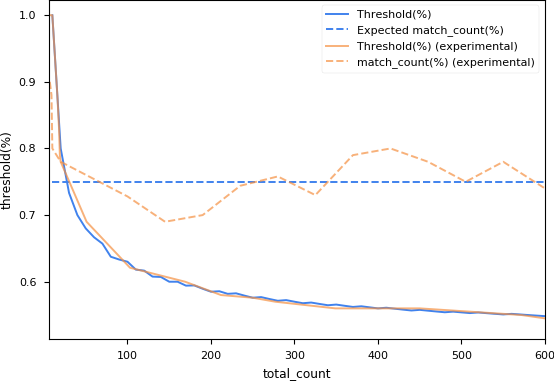
\includegraphics[width=\textwidth]{Figures/threshold_two-level.png}
    \caption{Portion of match\_count and \textit{threshold} for different total\_count to achieve the ownership confidence level 99\% ($\alpha_1=0.01$)}
    \label{fig:threshold-ownership}
\end{figure}

\Cref{fig:threshold-ownership} shows, for a fixed $\alpha_1=0.01$, the thresholds for different values of $total\_count$ as a fraction of $total\_count$ (continuous blue line).
The dashed blue line is the expected fraction of $match\_count$ out of $total\_count$ (75\%).
We can see that for the $total\_count$ larger than $\approx 30$ the previously mentioned condition is satisfied and the extraction algorithm can verify the ownership with a confidence level of 99\%. 
The statement is confirmed with the experimental results shown by the orange lines in the figure.
The experiments are run on Forest Cover Type data with fingerprint length $L=96$.
The $match\_count$ value in the experiments is $75\%(total\_count)\pm5\%$, according to the expectation. Furthermore, the lower limit for $total\_count$ to have 99\% confidence level for ownership is shown to be around 30. 
Therefore, \Cref{eq:ownership-verification} needs to be satisfied for the correct ownership verification.

\begin{equation}\label{eq:ownership-verification}
    2\eta/\gamma_1 > 30 (\alpha_1=0.01)
\end{equation}

For the real-life datasets with hundreds or thousands of tuples this is rather easy to achieve (e.g. for Forest Cover Type data, setting $\gamma_1=200$ results in $total\_count \approx 5,800$).

The second phase of detection algorithm - the fingerprint extraction - identifies each bit individually from the associated group of tuples. 
The process of comparing the matching bits to the threshold value is in this phase controlled by $\alpha_2$.
If the number of matches of a single bit value is larger than the threshold, the bit is decided to be that value (conditions in lines 11 and 13 of \Cref{alg:two-level-extraction}).

\begin{figure}
\centering
    \subfloat[$\alpha_2=0.01$]{{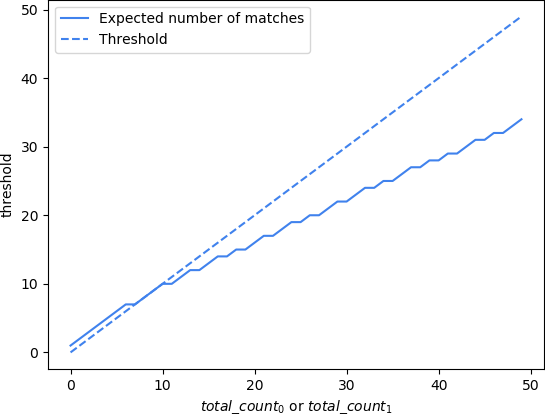
\includegraphics[width=6.7cm]{Figures/fingerprint-extraction-threshold-scrnsh.png} }}
    \qquad
    \subfloat[$\alpha_2=0.1$]{{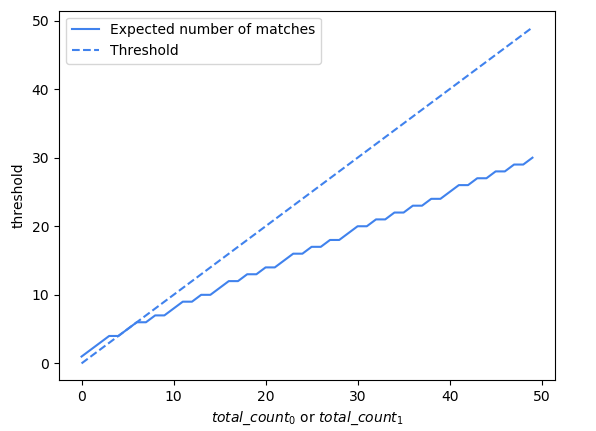
\includegraphics[width=6.7cm]{Figures/fingerprint-extraction-threshold-90.png} }}
    \caption{Threshold in subsets of unaffected marked data for different $total\_count_i$ to achieve confidence level of each bit of 99\% (a) and 90\% (b)}
    \label{fig:threshold-fingerprint-extraction}
\end{figure}

\Cref{fig:threshold-fingerprint-extraction} shows threshold values in a subset, depending on the total number of tuples in a subset. 
A dashed line represents the expected number of matches in a marked group of unaffected fingerprinted data.
We show the relation between thresholds and the number of matches for different levels of confidence - 99\% and 90\%.
Generally, the more tuples are selected into a subset, the more robust the fingerprint is. 
For reaching the confidence level of 99\%, $total\_count_i$  must be at least 8 for a trusted pattern to be found, while for 90\% confidence that lower limit is 4. 
Therefore, \Cref{eq:extraction-99} must be satisfied to obtain the successful marking pattern with confidence 99\% and \Cref{eq:extraction-90} with confidence 90\%.

\begin{equation}\label{eq:extraction-99}
    \eta/(\gamma_1 * L) > 7 (\alpha_2=0.01)
\end{equation}

\begin{equation}\label{eq:extraction-90}
    \eta/(\gamma_1 * L) > 3 (\alpha_2=0.1)
\end{equation}

In the real implementation $\eta/(\gamma_1 * L)$ should be rather larger than suggested in \Cref{eq:extraction-99,eq:extraction-90} because of the deviation introduced by random distribution of tuples into $L$ groups. 

\paragraph{}
The proposed technique has a limitation that it embeds the fingerprint in only one, initially chosen attribute. 
However, this approach is vulnerable to a vertical attack (attribute deletion attack) where the attacker can delete the fingerprint by removing the entire attribute. 
To avoid the possibility of such attack in multi-attribute datasets and for further experiments with this scheme, we slightly redesign the embedding and extraction process such that all attributes appear as candidates for marking. 
The simple modification is the reinterpretation of the term $LSB(r,j)$ in \Cref{alg:two-level-insertion}.
In this notation $LSB(r,j)$ represents the $j-th$ bit from the set of least significant bits available for marking of \textit{all} attribute values from the tuple $r$ (instead of only one predefined attribute).
Pseudo-randomness of this step ensures uniformly distributed marks over all attributes. 



\section{Fingerprinting categorical data}\label{subsec:fingerprinting-scheme-categorical}

We present two approaches to developing a technique that can be applied to both numerical and categorical data.
Both schemes use the processes of the AK Scheme for marking numerical values.
The first technique, a rather simplistic one, is based on a random choice of values to be marked and a random choice of a mark. 
In the second approach, we focus on keeping the semantic relations between the categorical data rather than purely randomly choosing the marks. 
The technique, however, relies on the availability of the original data, therefore, unlike the first scheme, it is not blind.
\paragraph{}
Another proposed technique for fingerprinting categorical data is \cite{Kieseberg2014fingerprinting}, where the $k$-anonymity pattern is used as a fingerprint. 
The number of $k$-anonymity patterns is limited and highly depends on the data and user-defined generalisation hierarchies, therefore also the number of distinct fingerprints is limited.
Furthermore, $k$-anonymity significantly changes the quality of the data. 
Since a subset of values is replaced by the respective value of the higher semantic category (e.g. Vienna->Austria), the informativeness of the data is lost.
Every buyer receives a distinct fingerprinted data copy, thus the quality of the data among the distributed copies differs significantly.
The technique lacks in implementation, therefore we do not include it in our analysis.

\subsection{Random mark choice}
\subsubsection{Methodology}
\paragraph{Insertion}
The approach for fingerprint embedding into the categorical data has the following steps:
\begin{enumerate}
    \item Label encoding all categorical values to obtain numerical data
    \item Fingerprint insertion algorithm of AK Scheme (Algorithm \ref{alg:AK-insertion})
    \item Applying modular arithmetic to fingerprinted numerical values of categorical data
    \item Decoding the values of categorical attributes
\end{enumerate}
The main idea of the approach is to convert categorical values to numerical values and treat them as any of the described methods for fingerprinting numerical data would. 
Assume that the attribute $A$ has $c$ different categorical values $C_0, ..., C_{c-1}$.
The label encoding model assigns each categorical value $C_i$ to the respective numerical value $i$.
After the fingerprint is embedded, the numerical values are being decoded back to the categorical values. 
A problem arises when a fingerprinted numerical value is not assigned to any of the categorical values in the encoding model because the range of values available in fingerprinting $2^\xi$, due to the binary representation, does not always correspond to the range of categorical values for an attribute.
The occurrence of such illegal values is possible when the fingerprint insertion algorithm marks a bit in the numerical representation of categorical value in such a way that the change of that bit transforms the numerical value to something that can't be decoded. 
For instance, assume that an attribute $A_1$ has 6 different categorical values ($c=6$), assigned by the encoding model to the numerical values $\{0,1,2,3,4,5\}$. 
Furthermore, assume $\xi=2$, and the insertion algorithm deciding to change the second least significant bit of value "4" somewhere within the dataset. 
The bit representation of the value $4_{10}=100_2$ will after marking be changed to $110_2$ which corresponds to $6$ in the decimal system, the value that is not assigned to any categorical value of attribute $A_1$. 
In general, the set of values of $A_1$ that can be obtained after embedding the fingerprint is $\{0,1,2,3,4,5,6,7\}$, where 6 and 7 are illegal values. 

Much bigger odds for a marked value to be out of bounds is in cases when the number of LSB-s available for fingerprinting $\xi$ is bigger than the length of bit representation the numerical values in label encoding model.
For example, assume $c = 4$, i.e. an attribute $A_2$ has 4 different values that are assigned to numerical values $\{0,1,2,3\}$, and $\xi = 3$. 
In case when insertion algorithm chooses, for example, value $2_{10}=10_2$ and its third least significant bit for fingerprinting, the resulting marked value is $110_2 = 6_{10}$, which does not have a corresponding categorical value in the encoding model. 
In general, after the fingerprint-embedding process, the domain of possible values of the attribute $A_2$ is $\{0,..,7\}$, where $\{4,5,6,7\}$ are not assigned to any original categorical value in our label encoding model. 

We solve the problem of illegal values in the fingerprinted dataset by applying modular arithmetic to the set of values obtained after fingerprinting. 
The final numerical value $x_i'$ of the attribute is given by $x_i' = x_i$ $mod$  $c$, where $x_i$ is the value after step 2 of the fingerprint-embedding process.
The modulo step in insertion algorithm for categorical data applied on $A_1$ would change the marked value $6_{10}=110_2$ to $6_{10} \mod 6 = 0_{10} = 000_2$. 

Finally, after removing the illegal values from the fingerprinted dataset, the numerical values are decoded to the categorical values. 

\paragraph{Detection}
Fingerprint detection process contains the following steps:
\begin{enumerate}
    \item Label encoding categorical values using the same model as in fingerprint insertion phase
    \item Fingerprint detection algorithm of AK Scheme (Algorithm \ref{alg:AK-detection})
\end{enumerate}

In the fingerprint detection process, it is again necessary to preprocess data by label encoding categorical values.
The encoding model needs to match the one from the insertion phase, otherwise, the detection process is disrupted.
After encoding categorical values, the AK detection algorithm \ref{alg:AK-detection} can be directly used to detect the malicious buyer.

\subsubsection{Properties and Discussion}
The properties of a detection algorithm for categorical data are essentially the same to the properties of AK detection algorithm, except that it is important to take into account the effects of modular arithmetic applied to the fingerprinted values where it is the case.
Consider the previous example with attribute $A_1$ where the fingerprint insertion algorithm changes the number representation $2_{10}=10_2$ of some categorical value to value $110_2 = 6_{10}$ by marking the third LSB and modulo operator application obtains the final marked value $6_{10} \mod 6 = 0_{10} = 000_2$. 
From this attribute value, the fingerprint bit cannot be correctly extracted anymore, therefore the detection algorithm is affected. 

The detection algorithm uses the technique called \textit{majority voting} for deciding the values of fingerprint bits, as discussed in \Cref{subsec:ak}.
This is the key to the property of the scheme that small errors in data do not prevent detecting the source of leakage. 
The effects of these small errors, i.e. values that are changed after inserting the fingerprint, are analysed in the context of attacks in \Cref{sec:Robustness}. 
Applying modulo to the values has the same effect on the detection process as purposely changing the values in fingerprinted data as part of a malicious attack (for example, bit flipping attack). 

 
The success of the detection process directly depends on the number of values that are a result of performing the modulo step in the insertion phase. 
This number is affected by the number of least significant bits we allow to change (parameter $\xi$) - larger $\xi$ leads to more frequent usage of modulo operation because the fingerprinted values more frequently get out of valid bounds. 
Since the detection process relies on multiple embeddings of a single fingerprint bit, having more marks in the dataset might assure that the fingerprint bits are detected correctly.
This is controlled by parameter $\gamma$ and the length of a fingerprint $L$.

\Cref{tab:detection-succ-german} presents the success of the detection algorithm for different values of parameters $\gamma$ and $\xi$. 
A fingerprint is in these experiments embedded in categorical values only.
Length of a fingerprint $L$ is set to 40.
The dataset used for experiments from \Cref{tab:detection-succ-german} is the German Credit data with 1000 entries and 21 attributes, out of which 14 are categorical. The dataset is described in \Cref{datasets}.
The results are based on 1000 runs of the algorithm for every parameter combination.

\begin{table}[ht]
    \centering
    \caption{Success of a detection algorithm of the fingerprinting scheme for categorical data using the German Credit dataset}
    \label{tab:detection-succ-german}
    \begin{tabular}{|c|r|r|r|r|}
    \hline
         & $\xi=1$ & $\xi=2$ & $\xi=4$ & $\xi=6$ \\
         \hline
         $\gamma=2$ & 99.8\% & 99.3\% & 56.4\% & 23.2\%\\
         \hline
         $\gamma=3$ & 94.7\% & 90.4\% & 17.3\% & 2.9\% \\
         \hline
         $\gamma=6$ & 30.0\% & 18.2\% & 0.3\% & 0\%\\
         \hline
         $\gamma=9$ &  2.9\% & 1.0\% & 0\% & 0\%\\
         \hline
         $\gamma=12$ & 0.1\% & 0\% & 0\% & 0\%\\
         \hline
    \end{tabular}
\end{table}

The detection algorithm performance significantly drops when either $\xi$ or $\gamma$ are increased. 
The expectation that the performance of the detection algorithm drops if more LSB-s are available for embedding the fingerprint (larger $\xi$) is confirmed by these experiments. 
\Cref{tab:german-credit} shows how many categorical attributes have a certain amount of different values in German Credit dataset. 
For instance, 3 out of 14 categorical attributes have 3 different values and therefore require only 2 bits to be encoded. 
An additional 10 attributes have up to 5 different values, therefore can be encoded by 3 bits. 


In the case where our insertion algorithm marks the 1st or the 2nd LSB of the value, the value obtained after fingerprinting will most likely be a modified numerical value that can be decoded back to a valid categorical value.
However, allowing e.g. the 4th significant bit to be marked in the insertion process opens more possibilities of obtaining values outside of the bounds, and modulo needs to be applied.
This results in the big decrease in the detection that can be seen in \Cref{tab:detection-succ-german} between $\xi=2$ and $\xi=4$. 
Applying modulo changes the marked value in the way that the detection algorithm can't extract the fingerprint bit correctly, leading to the impossibility of detecting a valid fingerprint. 
Generally, increasing $\xi$ leads to worse performance of the detection algorithm. 
A good choice for value of parameter $\xi$ depends very much on the dataset. 
One needs to inspect the dataset to see approximately how many different values the categorical attributes have, and set $\xi$ accordingly.
For example, if most of the categorical attributes have approximately 4 values, then $\xi$ should be at most 2 to keep the performance of the detection algorithm high. 
Generally, $\xi$ should be set to at most the number of bits needed to encode all the values of the attribute to their binary representations. 
The choice of parameter $\xi$ according to this will help in decreasing the loss in performance of the detection algorithm, but it generally cannot be completely avoided.
One of the reasons is that the choice of $\xi$ is limited to choosing the same value for the entire dataset, i.e. the same number of LSBs is available for fingerprinting in any of the attributes, no matter the size of their domains.
The optimal choice for $\xi$ from a detection performance point of view is then constrained by attributes with a small number of different values, while from the robustness point of view it is desired to have larger $\xi$, as discussed in detail in \Cref{sec:Robustness}. 
On the other hand, if the numbers of different values in all categorical attributes are not all power of two and $\xi$ not set according to the size of the smallest domain, there will always be even a minor possibility that the \textit{modulo} will be applied and will affect the detection algorithm. 

Besides the parameter $\xi$, the parameter $\gamma$ affects the performance of the detection algorithm, as shown in \Cref{tab:detection-succ-german} ($\gamma=2$ means that on average every second tuple is chosen for fingerprinting). 
Experiments show a significant decrease in performance when increasing $\gamma$. 
Increasing $\gamma$ means marking fewer tuples. Consequently, each fingerprint bit will be embedded in the data fewer times. 
This makes it harder for the detection algorithm to extract the correct value of a specific fingerprint bit when errors caused by the modulo operation are introduced. 
The design of our detection algorithm requires the perfect match of the fingerprint extracted by detection algorithm to some valid buyer's fingerprint, therefore only one falsely extracted fingerprint bit is enough for detection algorithm to fail. 
This is the reason for the success of 0\% for experiments with both high $\gamma$ and high $\xi$.

The issue that arises when fingerprinting dataset as small as German Credit data with only 1000 rows is that with $\gamma$ large enough, some fingerprint bits don't get embedded at all in the insertion process. 
Let us have an example where $\gamma=12$ and $L=40$. 
According to the parameters, $1000/\gamma \approx 83$ rows will be fingerprinted, and each fingerprint bit will be embedded into the dataset $83/40\approx2$ times. 
This number is approximate, and most importantly, averaged over all fingerprint bits. 
Since the choice of fingerprint bit to be embedded is completely independent and random in every step of the insertion algorithm, it is plausible to expect some bits being embedded 0 times.
This means that the detection algorithm will fail to extract the valid fingerprint from the unchanged fingerprinted dataset if the insertion process failed to embed all fingerprint bits at least once.
This observation is important to be noted when analyzing results from the \Cref{tab:detection-succ-german} because the success of the detection algorithm in small datasets is affected not only by errors caused by modulo operation but also by the failure of insertion algorithm to embed all of the fingerprint bits for larger $\gamma$.
To analyze these effects as separate cases, we define the following measures:
\begin{itemize}
    \item \textit{DFR} (Detection Fail Rate) - the number of fingerprint bits wrongly extracted because of the errors caused by modulo operation in the fingerprint detection process
    \item \textit{IFR} (Insertion Fail Rate) - the number of fingerprint bits that were not embedded at all in the fingerprint insertion process, and are therefore impossible to be extracted (unknown bit value)
    \item \textit{DIFF} - bit difference between the extracted fingerprint and the correct one; $DIFF = DFR + IFR$
\end{itemize}
\Cref{tab:detection-fail-rates} shows the rates obtained by the experiments shown in the \Cref{tab:detection-succ-german}, and presents a comparison of how much effect on the success of detecting the valid fingerprint is due to the modulo operation, and how much due to non-embedded bits. 
Rates in the table are the average values of rates from all 1000 runs. 
Insertion Fail Rate (\textit{IFR}) depends only on the number of dataset values being fingerprinted, i.e. parameter $\gamma$.
For $\gamma$ as small as two, a single fingerprint bit is embedded $1000/(\gamma * L) \approx 13$ times on average, and experimental results show that the insertion algorithm does not fail in embedding all of the fingerprint bits in any of the 1000 trials. 
The detection algorithm is, for $\gamma=2$, affected only by errors induced by modulo, and the fingerprint extracted by the algorithm and the correct one differ in only 0.002 bits on average.
For $\gamma = 12$ the \textit{IFR} raises up to $\approx5 / 40$, i.e. on average 5 out of 40 bits of the extracted fingerprint are incorrect.
From the experiments, we can see that in most of the cases $DFR$ is larger than $IFR$, i.e. errors in fingerprint extraction are mostly caused by applying modulo operation, except for small values of $\xi$. 

\begin{table}[ht]
    \centering
    \caption{Bit difference and the detection fail rates for the German Credit data}
    \label{tab:detection-fail-rates}
    \resizebox{\textwidth}{!}{
    \begin{tabular}{|c|r|r||r|r||r|r||r|r||r|r||r|}
    \hline
         & \multicolumn{2}{c||}{$\xi=1$} & \multicolumn{2}{c||}{$\xi=2$} & \multicolumn{2}{c||}{$\xi=4$} & \multicolumn{2}{c||}{$\xi=6$} &  \\
         \hline
         & $DIFF$ & $DFR$ & $DIFF$ & $DFR$ & $DIFF$ & $DFR$ & $DIFF$ & $DFR$ & $IFR$ \\
         \hline
          $\gamma=2$ & $ 0.002$& $  0.002$ & $ 0.007$ & $  0.007$ & $ 0.562$ & $  0.562$  &  $ 1.376$
             & $  1.376$ & 0\\
         \hline 
         $\gamma=3$ & $ 0.055$ & $  0.045$ & $ 0.100$ & $  0.090$  & $ 1.654$ & $  1.644$ & $ 3.203$ & $  3.193$
              & 0.010 \\
         \hline
         $\gamma=6$ & $1.170$ & $0.558$ & $1.642$ & $1.030$ & $5.603$ & $4.991$ & $7.842$  & $7.230$ & 0.612 \\
         \hline
          $\gamma=9$ & $3.615$ & $ 1.105$ & $4.256$ & $1.746$ & $9.206$ & $ 6.696$ & $11.498$ & $ 8.988$ & 2.510 \\
         \hline
         $\gamma=12$ & $6.462$ & $ 1.424$ & $
         7.190$ & $ 2.152$ & $11.935$ & $6.897$ &  $14.095$ & $9.057$ & 5.038 \\
         \hline
    \end{tabular}}
\end{table}


\Cref{tab:detection-succ-german-without-modulo} shows the experimental results of the success of the detection algorithm when modulo is not applied, but illegal numerical values are left in the fingerprinted dataset. 
Experiments are as well run on the German Credit dataset, with 1000 runs for each parameter value. 
This table highlights the case of having a small dataset. 
The results show how limited the choice of parameter $\gamma$ is in these cases. 

\begin{table}[ht]
    \centering
    \caption{Success of a detection algorithm using the German Credit dataset without applying modulo operation}
    \label{tab:detection-succ-german-without-modulo}
    \begin{tabular}{|c|c|c|c|c|c|}
    \hline
         $\gamma=2$ & $\gamma=3$ & $\gamma=6$ & $\gamma=9$ & $\gamma=12$ & $\gamma=15$\\
         \hline
         100\% & 99.0\% & 54.5\% & 7.6\% & 0.6\%  & 0\%\\
         \hline
    \end{tabular}
\end{table}

We repeat the experiments on another, larger dataset in order to examine the effects of modulo operation on the detection process, without other side effects such as the insertion algorithm failure.
For the experiments, we use Adult dataset. 
The dataset originally has 32,561 rows that contain missing values.
We will not examine dealing with missing values, so for the experiments, we use the subset of 30,162 rows that do not contain any missing values.
\Cref{tab:detection-succ-adult} shows the experimental results of the success of the detection algorithm to recognise the correct malicious buyer.
the fingerprint length \textit{L} is set to 80.
The results in \Cref{tab:detection-succ-adult} are the percentage of successfully detected fingerprints out of 1000 runs for every parameter combination.

\begin{table}[ht]
    \centering
    \caption{Success of the detection algorithm using Adult dataset}
    \label{tab:detection-succ-adult}
    \begin{tabular}{|c|r|r|r|r|}
    \hline
         & $\xi=1$ & $\xi=2$ & $\xi=4$ & $\xi=6$ \\
         \hline
         $\gamma=3$ & 100\% & 100\% & 100\% & 100\% \\
         \hline
         $\gamma=6$ & 100\% & 100\% & 100\% & 100\%\\
         \hline
         $\gamma=12$ & 100\% & 100\% & 100\% & 99.5\%\\
         \hline
         $\gamma=25$ & 100\% & 100\% & 95.8\% & 64.0\% \\
         \hline
         $\gamma=50$ & 95.6\% & 72.6\% & 25.2\% & 1.4\% \\
         \hline
         $\gamma=100$ & 14.2\% & 3.0\% & 0\% & 0\% \\
         \hline
    \end{tabular}
\end{table}

Comparing the results from \Cref{tab:detection-succ-german} and \Cref{tab:detection-succ-adult} it can be observed that the detection algorithm performance improved a lot by having a larger dataset. 
For low $\gamma$ the performance is perfect or close to perfect. 
Again, increasing $\xi$ leads to worse performance of the detection algorithm since the modulo operation is required more and fingerprint bits are wrongly detected. 
In \Cref{tab:adult-detection-rates} we can see that the extracted fingerprint is very "close" to the valid one. 
For instance, in the case of $\gamma=50$ and $\xi=2$, the performance of the algorithm drops to 72.6\%, but the bit difference between the extracted and real fingerprint is on average 0.31 (\Cref{tab:adult-detection-rates}, $DIFF$ rate), meaning that for most of the remaining 27.4\% runs of the algorithm, the fingerprints' bit difference is only in one single bit. 
In \Cref{tab:adult-detection-rates} we omitted the experiments where the detection success is 100\% since all the rates for those cases are 0.
In other cases, we can see that insertion fail rate $IFR$ is very small or zero, so most of the fingerprint detection failure is caused by modulo operation. 

\begin{table}[ht]
    \centering
    \caption{The detection fail rates for Adult data}
    \label{tab:adult-detection-rates}
    \resizebox{\textwidth}{!}{
    \begin{tabular}{|c|r|r||r|r||r|r||r|r||r|r||r|}
    \hline
         & \multicolumn{2}{c||}{$\xi=1$} & \multicolumn{2}{c||}{$\xi=2$} & \multicolumn{2}{c||}{$\xi=4$} & \multicolumn{2}{c||}{$\xi=6$} &  \\
         \hline
         & $DIFF$ & $DFR$ & $DIFF$ & $DFR$ & $DIFF$ & $DFR$ & $DIFF$ & $DFR$ & $IFR$ \\
         \hline
        $\gamma=25$ & $ 0$  & $  0$  & $ 0$ &$  0$  & $ 0.043$ & $  0.043$ & $ 0.431$ & $  0.431$ & 0 \\
         \hline
         $\gamma=50$ & $ 0.047$ & $  0.003$ & $ 0.310$ & $  0.266$ & $ 1.302$ & $  1.258$  & $ 3.987$ & $  3.943$ & 0.044 \\
         \hline
         $\gamma=100$ & $ 1.994$ & $  0.158$ & $ 4.086$ & $  2.250$ & $ 7.030$ & $  5.194$ & $ 12.228$ & $  10.392$ & 1.836 \\
         \hline
    \end{tabular}}
\end{table}


The problem of having illegal categorical values after the fingerprinting process is thwarted by the solution that introduces another problem - the weaker performance of the detection algorithm. 
Bad performance of the detection algorithm necessarily means that the presented fingerprinting scheme for categorical data is more susceptible to the attacks.
Small datasets are more vulnerable because of the possibility that the insertion algorithm fails to embed the fingerprint properly, not only in the context of categorical data but in general.
By careful dataset inspection and parameter tuning, both problems of small dataset and errors caused by modulo can be avoided. 
Lower \textit{L}, $\gamma$ and $\xi$ in general lead to better performance.

\paragraph{}
We saw that the number of LSB-s $\xi$ defines the quality of the scheme and that by choosing smaller $\xi$ we can minimise the error of the detection algorithm. 
In the discussion above, we use the fixed $\xi$ for all the attributes. 
However, we could modify this property such that each attribute $A_i$ is associated with own $\xi_i$ based on the number of distinct values of that attribute. 
This way we increase the robustness by setting particular $\xi_i$ values as high as possible, taking into account the upper limit that is defined by the number of distinct values in the attribute. 
For instance, changing only one LSB in the attribute with only three values, but allowing to change 5 LSB-s in attributes with $>40$ values. 

This approach is simplistic but effective. 
We will see in \Cref{sec:Robustness} the robustness analysis of the scheme and in \Cref{chapter:Utility} the utility analysis.
Another aspect that could be taken into account when designing a robust fingerprint technique is the semantic correlation between the categorical attributes. 
For instance, the fingerprint might be much more perceptible when there is a frequent number of occurrences of impossible or very unlikely combinations of attribute values due to marking.
This problem is addressed in the following section.


\subsection{Choosing a mark based on correlations in the dataset}
This approach addresses the problem of semantic relations between categorical attributes that can be disturbed by fingerprinting. 
Considering attributes independently of each other and embedding a random mark into a categorical value might lead to non-consistent records. 
A mark may introduce an uncommon or impossible combination of values in the data. 
As an example, let us consider a dataset containing attributes \textit{gender}, \textit{numberOfPregnancies}, etc. The attributes \textit{gender} and \textit{numberOfPregnancies} intuitively contain an impossible combination of values: (\textit{gender}:male, \textit{numberOfPregnancies}:1).
Another example is where the combination of values might be very uncommon. Take, for example, a medical dataset containing information about the patients suffering from Alzheimer's disease. The combination 
(\textit{alzheimersStage}:middle, \textit{employed}:yes) is very uncommon, but might be introduced by a random fingerprint mark.
With a dataset domain knowledge, these examples would be rather suspicious and thus perceptible. 
We aim to take into account the correlation between the values of different attributes and avoid uncommon combinations. 
\Cref{alg:cat-insertion} shows the pseudocode for the insertion algorithm of the scheme.

\subsubsection{Methodology}
\paragraph{Insertion}
\begin{algorithm}
  \KwIn{dataset $\mathcal{R}$ with scheme $(P, A_{0}, ..., A_{v-1})$, buyer $n$'s ID $id$}
  \KwOut{fingerprinted dataset $\mathcal{R'}$}
  fingerprint of buyer $n$: $\mathcal{F}(\mathcal{K},id)=\mathcal{H}(\mathcal{K}|id)$
  \\
  \ForEach{tuple $r \in \mathcal{R}$}
  {
    \If{$(\mathcal{S}_{1}(\mathcal{K}|r.P)$ mod $\gamma == 0)$}{
        attribute\_index $i = \mathcal{S}_2(\mathcal{K}|r.P)$ mod $v$
        \\
        \uIf{$A_i$ is categorical}{
            mask\_bit $x=0$ if $\mathcal{S}_3(\mathcal{K}|r.P)$ is even; $x=1$ otherwise \\
            fingerprint\_index $l=\mathcal{S}_4(\mathcal{K}|r.P)$ mod $L$
            \\
            fingerprint\_bit $f=f_l$\\
            mark\_bit $m=x \oplus f$ \\
            \If{m == 1}{
                neighbourhood = $select\_neighbours()$ \\
                target\_values, freq = $get\_frequencies(\text{neighbourhood})$\\
                $r.A_i = random(\text{target\_values}, weight=\text{freq})$
            }
        }
        \uElseIf{$A_i$ is numerical}{
            bit\_index $j=\mathcal{S}_3(\mathcal{K}|r.P)$ mod $\xi$
            \\
            mask\_bit $x=0$ if $\mathcal{S}_4(\mathcal{K}|r.P)$ is even; $x=1$ otherwise
            \\
            fingerprint\_index $l=\mathcal{S}_5(\mathcal{K}|r.P)$ mod $L$
            \\
            fingerprint\_bit $f=f_l$
            \\
            mark\_bit $m=x \oplus f$
            \\
            $LSB(j,r.A_i) = m$
        }
    }
  }
  \Return{$\mathcal{R'}$}
  \caption{Fingerprinting technique for categorical data: Insertion Algorithm}
  \label{alg:cat-insertion} 
\end{algorithm}

The insertion algorithm resembles the AK Scheme's insertion algorithm (\Cref{alg:AK-insertion}).
The creation of a fingerprint and the pseudorandom choice of tuples and attributes to be marked is the same.
In this scheme, the distinction is made based on whether a numerical or a categorical attribute is chosen for fingerprinting (line 5). 
In a case where the attribute is categorical, the next random value generated by a pseudorandom number generator $\mathcal{S}$ decides the value of a mask bit $x$. 
Furthermore, the next random value from the generator decides which fingerprint bit $f_l$ is going to be embedded. 
The mark bit $m$ is a result of an XOR operation between the mask and the fingerprint bit. 
In case the mark is 1, the attribute value will be marked. 
The lines 11 to 13 of \Cref{alg:cat-insertion} are specific for this scheme and contain the main part of this scheme.
Instead of marking the value to something random from the domain of the attribute, the idea is to choose a value taking into account the values of the other attributes in the tuple. 
This way, the algorithm avoids the combinations of values that are unlikely to appear in the dataset. 
We search for a neighbourhood of the observed tuple regarding all attributes but one that is being fingerprinted. 
We find the neighbours using the nearest neighbours algorithm with the Hamming distance. 
We let the user select whether the neighbourhood will be defined as a certain number of neighbours, $k$, or as the set of elements within the given distance $d$.
The parameters $k$ and $d$ are predefined by the user as well. 
After the neighbours are obtained, we observe the values in the attribute $A_i$ and sort them by their frequencies. 
The new value, i.e. the fingerprinted value is then a random value from the set of neighbours' values, where the random choice is weighted by values' frequencies. 
This technique is known in genetic algorithms as a fitness proportionate selection, or roulette wheel selection, a genetic operator used for selecting potentially useful solutions for recombination.
Fingerprinting process of numerical values follows the steps of the AK Scheme. 

\paragraph{Detection}
The pseudocode for the detection algorithm is shown in \Cref{alg:cat-detection}.

\begin{algorithm}
  \KwIn{fingerprinted dataset $\mathcal{R'}$ with scheme $(P, A_0, ..., A_{v-1})$, original dataset $\mathcal{R}$ with scheme $(P,A_0,...,A_{v-1}$}
  \KwOut{suspected buyer's ID $id$}
  fingerprint template $\mathcal{F}=(f_0,...,f_{L-1})=(?,...,?)$  \\
  $count[i][0]=count[i][1]=0$ \textbf{for} $i=0$ to $L-1$\\ 
  \ForEach{tuple $r \in R'$}
  {
    \If{$\mathcal{S}_1(\mathcal{K},r.P)$ mod $\gamma==0$}
    {
        attribute\_index $i=\mathcal{S}_2(\mathcal{K},r.P)$ mod $v$\\
        \uIf{$A_i$ is categorical}{
            mask\_bit $x=0$ if $\mathcal{S}_3(\mathcal{K},r.P)$ is even; $x=1$ otherwise\\
            \uIf{$r.A_i$ is different from the original}{
                mark\_bit $m = 1$
            }
            \uElse{
                mark\_bit $m= 0$
            }
            fingerprint\_index $l=\mathcal{S}_4(\mathcal{K},r.P)$ mod $L$\\
        }
        \uElseIf{$A_i$ is numerical}{
        bit\_index $j=\mathcal{S}_3(\mathcal{K}, r.P)$ mod $v$\\
        mark\_bit $m=LSB(j, r.A_i)$\\
        mask\_bit $x=0$ if $\mathcal{S}_4(\mathcal{K},r.P)$ is even; $x=1$ otherwise\\
        fingerprint\_index $l=\mathcal{S}_5(\mathcal{K},r.P)$ mod $L$\\
        }
        //update the votes\\
        fingerprint\_bit $f=m \oplus x$\\
        $count[l][f]++$ 
    }
  }
  //recover the fingerprint\\
  \For{$l=0$ to $L-1$}
  {
    \If{$count[l][0]+count[l][1]==0$}
    {
        \Return{\textit{none suspected}}
    }
    $f_l=0$ if $count[l][0]/(count[l][0]+count[l][1])>\tau$\\
    $f_l=1$ if $count[l][1]/(count[l][0]+count[l][1])>\tau$\\
    \Return{\textit{none suspected}} otherwise
  }
  $\mathcal{F}=(f_0,...,f_{L-1})$\\
  $id=detect(\mathcal{F,K},L, N)$\\
  \uIf{$id\geq0$}
  {
    \Return{$id$}
  }
  \Else
  {
    \Return{\textit{none suspected}}
  }
  \caption{Fingerprinting technique for categorical data: Detection Algorithm}
  \label{alg:cat-detection}
\end{algorithm}

Similarly to the AK's detection algorithm (\Cref{alg:AK-detection}), the algorithm starts by initializing the fingerprint template and the votes for fingerprint bit values. 
We then find the tuples and attributes that should have been fingerprinting according to the same pseudorandom sequence as in the insertion algorithm. 
For categorical attributes, the fingerprint extraction is described from line 7 to 12. 
We retrieve the mask bit $x$.
Next, to find the value of the mask bit $m$, it is necessary to compare the suspected fingerprinted dataset to the original. 
If the corresponding value is different from the original, then the value $m$ was 1 in the insertion algorithm, otherwise 0. 
Furthermore, we find the fingerprint bit index $l$ as the next random value in the pseudorandom sequence generator.
The lines 13 to 17 contain the extraction from the numerical values which is the same as in the extraction algorithm of the Ak Scheme.
The lines 18 to 38 are common for both categorical and numerical data and follow the steps from the detection algorithm of the AK Scheme. 

\subsubsection{Discussion}
Neighbourhood search is implemented in two different ways and is left to the user to decide which one to use for the specific case. We allow searching for a fixed number of neighbours, $k$, or searching for neighbours within a predefined distance $d$. 
The choice between the approach, as well as setting the parameters $k$ and $d$ requires some expert knowledge about the dataset. 
In case of an approach based on selecting a fixed number of neighbours, it is important to handle the neighbours with the same distances deterministically. We solve this in the following way: first, we choose the $k$ neighbours, then find the maximum distance within the neighbours and select all elements outside of the neighbourhood with the same distance. 
Therefore, it might be the case where the neighbourhood is extended to more than $k$ elements.

The set of attributes included in the neighbourhood selection do not have to be the whole set of attributes of the dataset. 
This can be set by the user who has insights into the data and has the knowledge about the highly related attributes. 

The final choice of the mark could be ambiguous if we would always choose the most frequent ones, in cases when we have multiple values with the same frequencies. 
For that reason we choose to select the new value pseudorandomly, weighted by the frequencies. This way the whole set of values from the neighbourhood have a chance to be selected, while the most frequent one will be selected with the highest probability.



\section{Summary}
In this chapter we have presented three common fingerprinting techniques for fingerprinting relational datasets, the AK Scheme in \Cref{subsec:ak}, Block Scheme in \Cref{subsec:block-oriented-scheme} and Two-level Scheme in \Cref{sec:two-level-fp}. 
These techniques have in common the usage of cryptographically secure structures and algorithms, i.e. cryptographic pseudo-random sequence generator and cryptographic hash function. They are used for creating the buyers' fingerprints because of security reasons since they must remain secret to everyone except the owner of the dataset. 
These techniques are limited to application on numerical values in the data. 
Furthermore, two fingerprinting techniques for non-numerical data are introduced in \Cref{subsec:fingerprinting-scheme-categorical}.
Both techniques extend the AK Scheme such that the same algorithmic steps are used for fingerprinting the numerical part of the data. 
The first scheme follows the pseudo-random pattern of choosing marks for categorical values.
In the second scheme, the solution goes towards preserving the correlations between the categorical values and marks the values in a way that no uncommon combinations of values occur in the final fingerprinted copy of the dataset.

These techniques are the basis of the analysis in the following chapters. The techniques are susceptible to attempts of a malicious buyer to destroy the fingerprint from the dataset. 
In the next chapter, we analyse how robust these techniques are under certain types of attacks.
